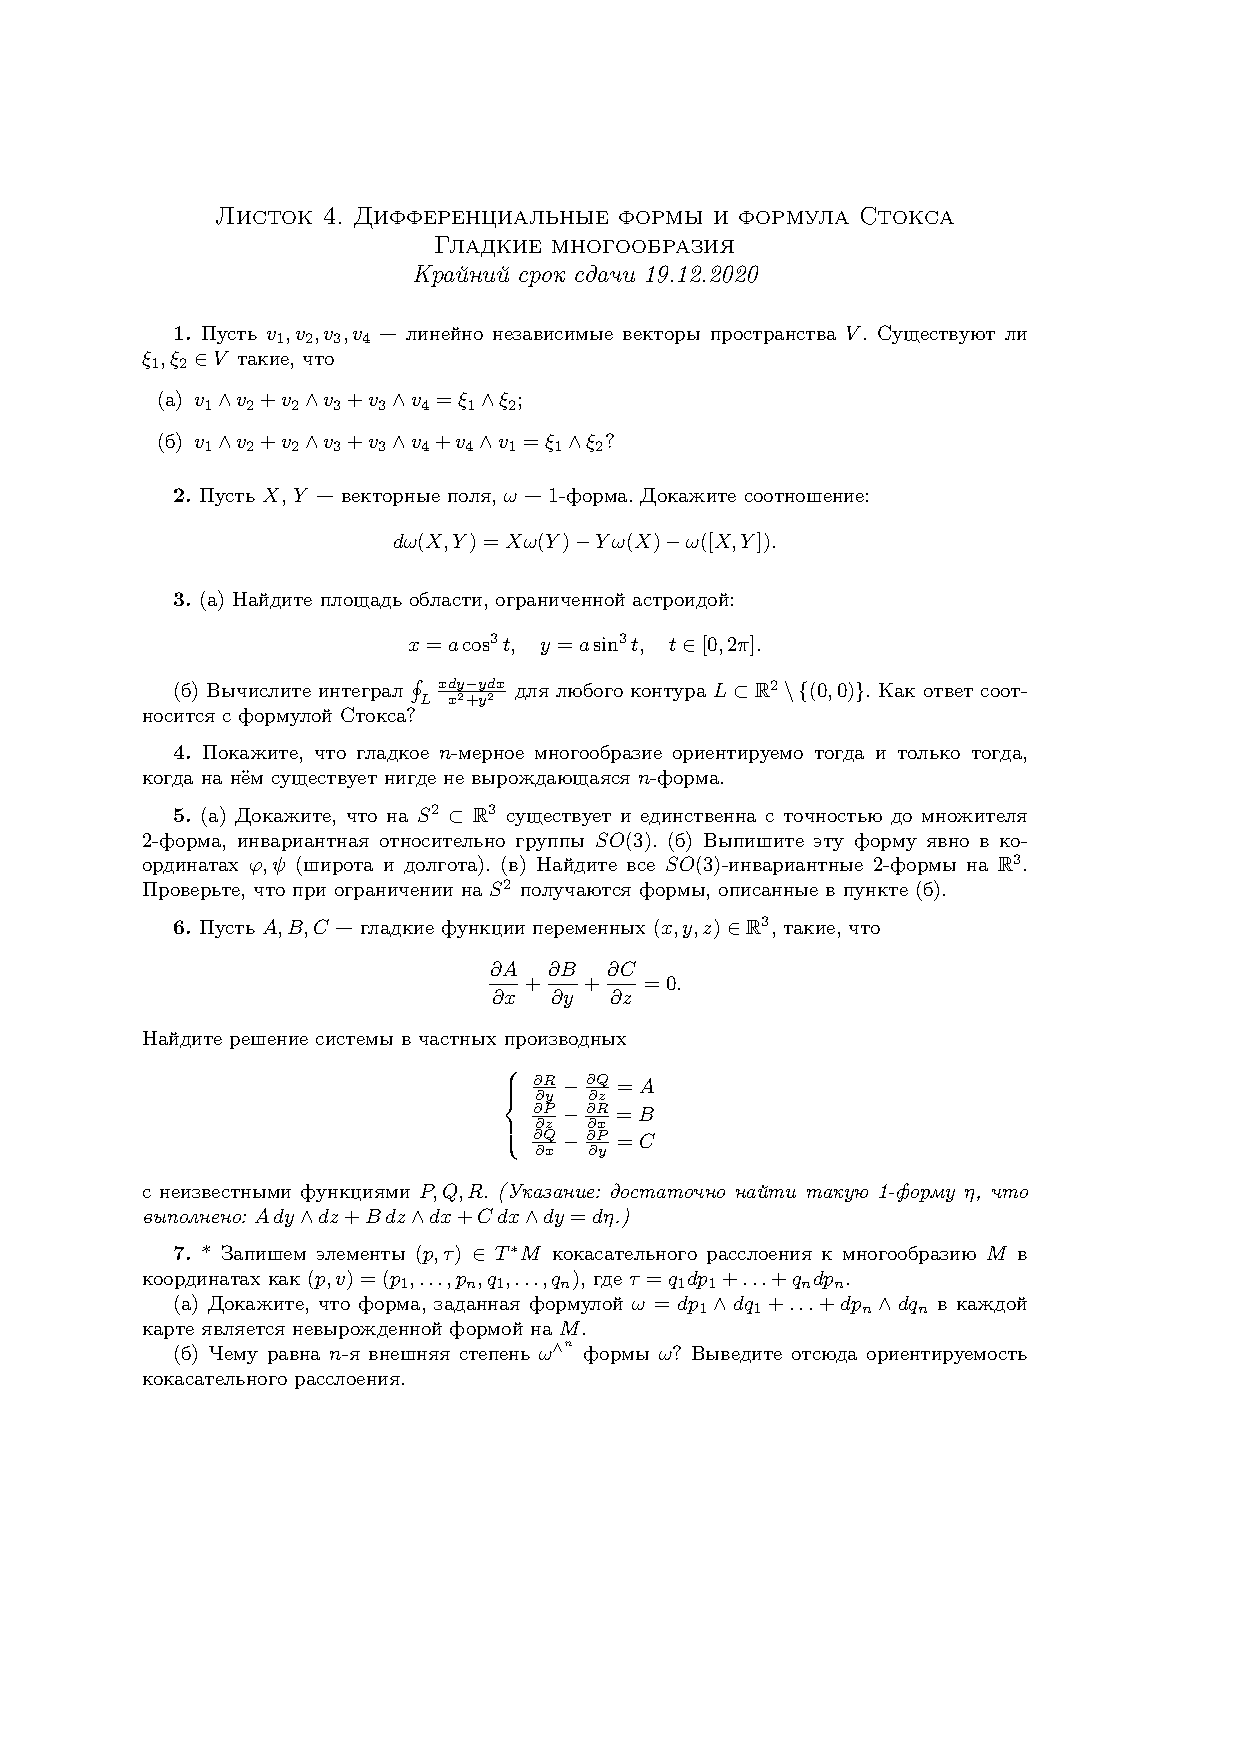
\includepdf[scale=0.95,pages=1,pagecommand=\section*{Условия}]{Tasks/Probl-manif4}
\newpage
\section*{Решения}
\subsection*{Задача 1}
\begin{enumerate}
\item[(а)]
	\begin{gather*}
		\xi_1 = \alpha_1 v_1 + \beta_1 v_2 + \gamma_1 v_3 + \delta_1 v_4\\
		\xi_2 = \alpha_2 v_1 + \beta_2 v_2 + \gamma_2 v_3 + \delta_2 v_4\\
		\\
		\xi_1 \wedge \xi_2 = \\
		\alpha_1 \beta_2 v_1 \wedge v_2 + \alpha_1 \gamma_2 v_1 \wedge v_3 + \alpha_1 \delta_2 v_1 \wedge v_4 + \beta_1 \alpha_2 v_2 \wedge v_1 + \beta_1 \gamma_2 v_2 \wedge v_3 + \beta_1 \delta_2 v_2 \wedge v_4 +\\
		 \gamma_1 \alpha_2 v_3 \wedge v_1 + \gamma_1 \beta_2 v_3 \wedge v_2 + \gamma_1 \delta_2 v_3 \wedge v_4 + \delta_1 \alpha_1 v_4 \wedge v_1 + \delta_1 \beta_2 v_4 \wedge v_2 + \delta_1 \gamma_2 v_4 \wedge v_3 =\\
		\\
		(\alpha_1 \beta_2 - \beta_1 \alpha_2) v_1 \wedge v_2 + (\alpha_1 \gamma_2 - \gamma_1 \alpha_2) v_1 \wedge v_3 + (\alpha_1 \delta_2 - \delta_1 \alpha_2)v_1 \wedge v_4\\
		+ (\beta_1 \gamma_2 - \gamma_1 \beta_2) v_2 \wedge v_3 + (\beta_1 \delta_2 - \delta_1 \beta_2) v_2 \wedge v_4 + (\gamma_1 \delta_2 - \delta_1 \gamma_2) v_3 \wedge v_4 =\\
		\\
		v_1 \wedge v_2 + v_2 \wedge v_3 + v_3 \wedge v_4\\
		\begin{cases}
			\alpha_1 \beta_2 - \beta_1 \alpha_2 = 1\\
			\alpha_1 \gamma_2 - \gamma_1 \alpha_2 = 0\\
			\alpha_1 \delta_2 - \delta_1 \alpha_2 = 0\\
			\beta_1 \gamma_2 - \gamma_1 \beta_2 = 1\\
			\beta_1 \delta_2 - \delta_1 \beta_2 = 0\\
			\gamma_1 \delta_2 - \delta_1 \gamma_2 = 1
		\end{cases}
	\end{gather*}
	Откуда следует
	\begin{gather*}
		\frac{\alpha_1}{\alpha_2} = \frac{\gamma_1}{\gamma_2} = \frac{\delta_1}{\delta_2}\ \Rightarrow\ \gamma_1 \delta_2 - \delta_1 \gamma_2 = 0\quad \text{но } \gamma_1 \delta_2 - \delta_1 \gamma_2 = 1
	\end{gather*}
	Следовательно такой пары $\xi_1, \xi_2$ не существует
\item[(б)]
	\begin{gather*}
		v_1 \wedge v_2 + v_2 \wedge v_3 + v_3 \wedge v_4 + v_4 \wedge v_1 =\\
		v_1 \wedge v_2 - v_3 \wedge v_2 + v_3 \wedge v_4 - v_1 \wedge v_4 =\\
		(v_1 - v_3) \wedge (v_2 - v_4) = 
		\xi_1 \wedge \xi_2
	\end{gather*}
\end{enumerate}
\vskip 0.4in


\subsection*{Задача 2}
	Пусть $\omega = fdg,\ f,g \in C^{\infty}(U)$, тогда $d \omega = d(fdg) = df \wedge dg$, тогда
	\begin{gather*}
	d \omega (X,Y) = df(X)dg(Y) - df(Y)dg(X) = (Xf)Yg - (Yf)Xg\\
	X \omega (Y) = X(fdg(Y)) = X(fYg) = (Xf)Yg + fXYg\\
	Y \omega (X) = Y(fdg(X)) = Y(fXg) = (Yf)Xg + fYXg\\
	\omega ([X,Y]) = fdg([X,Y]) = f(XY - YX)g
	\end{gather*}
	Откуда следует
	\begin{gather*}
	X \omega (Y) - Y \omega (X) - \omega ([X,Y]) = (Xf)Yg - (Yf)Xg = d \omega (X,Y)
	\end{gather*}
\vskip 0.4in
\begin{comment}
	\begin{gather*}
	(dw)(X_0,\ldots,X_n) = \sum\limits_{i=0}^{n} (-1)^i X_i (w(X_0,\ldots,\hat{X}_i,\ldots,X_n)) +\\
	\sum\limits_{0 \leqslant i < j \leqslant n} (-1)^{i+j}w([X_i,X_j],X_0,\ldots,\hat{X}_i,\ldots,\hat{X}_j,\ldots,X_n)
	\end{gather*}
	Тогда
	\begin{gather*}
	dw(X,Y) = (i_X dw)(Y) = (L_X w)(Y) - (dw(X))(Y)
	\end{gather*}
	И так как $L_X$ коммутирует с сжимающим оператором,то
	\begin{gather*}
	Xw(Y) = L_X(w(Y)) = (L_X w)(Y) + w([X,Y])\ \Leftrightarrow\ (L_X w)(Y) = Xw(Y) - w([X,Y])
	\end{gather*}
	Тогда
	\begin{gather*}
	dw(X,Y) = Xw(Y) - w([X,Y]) - (dw(X))(Y) = Xw(Y) - Yw(X) - w([X,Y])
	\end{gather*}
\end{comment}


\subsection*{Задача 3}
\begin{enumerate}
\item[(а)]
	\begin{gather*}
	\begin{cases}
	x = a \cos(t)^3\\
	y = a \sin(t)^3
	\end{cases}\\
	S = 
	4\int_{0}^{a} y dx =
	4\int_{x = 0}^{x = a} y \frac{dx}{dt} dt =\\
	4\int_{x = 0}^{x = a} a\sin(t)^3 3a\cos(t)^2 \sin(t) (-\sin(t)) dt =\\
	4\int_{t = \frac{\pi}{2}}^{t = 0} a\sin(t)^3 3a\cos(t)^2 \sin(t) (-\sin(t)) dt =\\
	12a^2 \int_{0}^{\frac{\pi}{2}} \sin(t)^4 \cos(t)^2 dt
	\end{gather*}
	Распишем $\sin(t)^4\cos(t)^2$
	\begin{gather*}
	\sin(t)^4\cos(t)^2 = 
	\frac{(2\sin(t)\cos(t))^2}{4} \cdot \frac{2\sin(t)^2}{2} =\\
	\frac{\sin(2t)^2}{4} \cdot \frac{2\sin(t)^2}{2} =
	\frac{\sin(2t)^2}{4} \cdot \frac{1 - \cos(2t)}{2} =\\
	\frac{\sin(2t)^2 - \sin(2t)^2\cos(2t)}{8} =
	\frac{1 - \cos(4t)}{16} \cdot \frac{\sin(2t)^2} \cos(2t){8}
	\end{gather*}
	Тогда
	\begin{gather*}
	S = 
	12a^2 \int_{0}^{\frac{\pi}{2}} \left(\frac{1 - \cos(4t)}{16} - \frac{\sin(2t)^2 \cos(2t)}{8}\right) dt =\\
	\frac{3}{4}a^2 \int_{0}^{\frac{\pi}{2}}(1-\cos(4t))dt - \frac{3}{2}a^2 \int_{0}^{\frac{\pi}{2}} \sin(2t)^2 \cos(2t) dt =\\
	\frac{3}{4}a^2 \left(t - \frac{\sin(4t)}{4}\right)\bigg|_{0}^{\frac{\pi}{2}} - \frac{3}{2}a^2 \left(\frac{\sin(2t)^3}{6}\right) \bigg|_{0}^{\frac{\pi}{2}} =\\
	\frac{3\pi a^2}{8} - \frac{3a^2}{16}\sin(2\pi) - \frac{3a^2}{12}\sin(\pi)^3 =
	\frac{3\pi a^2}{8}
	\end{gather*}
\item[(б)]
	Заметим, что $\frac{xdy - ydx}{x^2 + y^2}$ -- производная $\arctan(\frac{x}{y})$, тогда
	\begin{gather*}
	\oint_L \frac{xdy - ydx}{x^2 + y^2} = \arctan\left(\frac{x}{y}\right)\bigg|_{(x_1,y_1)}^{(x_2,y_2)}
	\end{gather*}
	Разобьем контур на отрезки, на которых нет точек пресечения. Тогда будем интегрировать по промежуткам $(t_1, t_2)$, где $x(t_1) = x(t_2),\ y(t_1) = y(t_2)$. Вычислим значения на промежутках через замену $x(t) = \sin(\varphi),\ y(t) = \cos(\varphi)$, откуда
	\begin{gather*}
	\arctan\left(\frac{x(t)}{y(t)}\right) \bigg|_{t_2}^{t_1} = \varphi|_{s_1 + 2\pi}^{s_1} = 2\pi\\
	\oint_L \frac{xdy - ydx}{x^2 + y^2} = 2\pi k\quad \text{где } k \text{ -- степень отображения}
	\end{gather*}
	
	
	
\end{enumerate}
\begin{comment}
	Зададим контур параметрически
\begin{gather*}
(x(t), y(t)),\ t \in [0,1]\\
\int_{0}^{1} \frac{x(t) y'(t) - y(t) x'(t)}{x^2(t) + y^2(t)}dt = 
\int_{0}^{1} \left(\frac{x(t)}{y(t)}\right)' \cdot \frac{y^2(t)}{x^2(t) + y^2(t)}dt =
\int_{0}^{1} \left(\frac{x(t)}{y(t)}\right)' \cdot \frac{1}{\left(\frac{x(t)}{y(t)}\right)^2 + 1} dt
\end{gather*}
Разобьем $[0,1]$ на интервалы, для каждого из которых выполнено, что $\left(\frac{x(t_1)}{y(t_1)}\right) \ne \left(\frac{x(t_2)}{y(t_2)}\right)$ при $t_1 \ne t_2$. Тогда
\begin{gather}
\int_{0}^{1} \frac{1}{\left(\frac{x(t)}{y(t)}\right)^2 + 1} d\left(\frac{x(t)}{y(t)}\right) = \sum \int \frac{1}{\left(\frac{x(t)}{y(t)}\right)^2 + 1} d\left(\frac{x(t)}{y(t)}\right) = \sum \arctan\left(\frac{x(t)}{y(t)}\right)
\end{gather}
По формуле стокса, если контур замкнут, то интеграл равен 0, иначе, если контур не замкнут, он не равен 0

\oint_L \frac{xdy - ydx}{x^2 + y^2} = 
\oint_L \left(\frac{x}{x^2 + y^2}dy - \frac{y}{x^2 + y^2}dx\right) =\\
\oint_L \left(\frac{M}{dx} + \frac{N}{dy}\right)\qquad M = \frac{-y}{x^2 + y^2},\ N = \frac{x}{x^2 + y^2}\\
\iint_D \left(\frac{M}{dx} + \frac{N}{dy}\right)dxdy = 
\iint_D \frac{M}{dx}dxdy + \iint_D \frac{N}{dy}dxdy =
\end{comment}
\vskip 0.4in


\subsection*{Задача 4}
	Пусть $\mu$ -- нигде не вырождающаяся $n$-форма на многообразии $M$. Тогда для каждой локальной карты $(U,x^{1},\ldots,x^{n})$ существует гладкая функция $f \ne 0$, такая что $\mu = fdx^{1} \wedge \ldots \wedge dx^{n}$. Тогда $\mu(\partial_1,\ldots,\partial_n) = f \ne 0$.\\
	Тогда мы можем для каждой точки найти карту, для которой $f > 0$ (рассмотрев любую карту и заменив $x^{1}$ на $-x^{1}$ если $f < 0$). Тогда рассмотрим 2 пересекающихся карты $(U_{\alpha},x^{1}_{\alpha},\ldots,x^{n}_{\alpha})$ и $(U_{\beta},x^{1}_{\beta},\ldots,x^{n}_{\beta})$, ддя их пересечения выполнено:
	\begin{gather*}
		\mu = f dx^{1}_{\alpha} \wedge \ldots \wedge dx^{n}_{\alpha} = gdx^{1}_{\beta} \wedge \ldots \wedge dx^{n}_{\beta}\qquad f,g > 0\\
		0 < g = \mu(\partial_1^{\beta},\ldots,\partial_n^{\beta})^= (\det d\phi_{\alpha \beta}) \mu(\partial_1^{\alpha},\ldots,\partial_n^{\alpha}) = (\det d\phi_{\alpha \beta})f
	\end{gather*}
	Откуда следует что $\det(d\phi_{\alpha \beta}) > 0$ тогда построенный таким образом атлас будет иметь ориентацию
	\vskip 0.2in
	Пусть $A$ -- ориентация, тогда для каждой карты $U_{\alpha}$ с $A$ предположим что $\mu_{\alpha} = dx^{1}_{\alpha} \wedge \ldots \wedge dx^{n}_{\alpha}$. Рассмотрим тогда $\{\rho_{\alpha}\}$, . Тогда $\mu := \sum\limits_{\alpha} \rho_{\alpha} \mu_{\alpha}$ нигде не вырождающаяся гладкая $n$-форма на $M$. Тогда для каждого $p \in M$ существует окрестность $U$ такая что $\sum\limits_{\alpha} \rho_{\alpha} \mu_{\alpha}$ -- конченая сумма $\sum\limits_{i = 1}^{k} \rho_{i} \mu_{i}$, тогда в окрестности $p$
	\begin{gather*}
		\mu(\partial_1^1,\ldots,\partial_n^{1}) = \sum\limits_{i = 0}(\det d \phi_{1k})\rho_{i} > 0\ \Leftrightarrow \mu \ne 0
	\end{gather*}
\vskip 0.4in %http://staff.ustc.edu.cn/~wangzuoq/Courses/18F-Manifolds/Notes/Lec23.pdf


\subsection*{Задача 5}
	Рассмотрим $\omega = z dx \wedge dy + y dz \wedge dx + x dy \wedge dz$, проверим что такая форма подходит
	\begin{gather*}
		A = 
		\begin{pmatrix}
			a_1 & b_1 & c_1\\
			a_2 & b_2 & c_2\\
			a_3 & b_3 & c_3
		\end{pmatrix}
		\in SO(3)\qquad \det(A) = 1\\
		x' = a_1 x  + b_1 y + c_1 z\\
		y' = a_2 x  + b_2 y + c_2 z\\
		z' = a_3 x  + b_3 y + c_3 z\\
		\omega(x',y',z') = 
		z'dx' \wedge dy'+ y'dz' \wedge dx' + x'dy' \wedge dz' =\\
		\left(a_3x + b_3y + c_3z\right)\left(\left(a_1b_2 - a_2b_1\right)dx \wedge dy + \left(b_1c_2 - b_2c_1\right)dy \wedge dz + \left(c_1a_2 - c_2a_1\right)dz \wedge dx\right) +\\
		\left(a_2x + b_2y + c_2z\right)\left(\left(a_3b_1 - a_1b_3\right)dx \wedge dy + \left(b_3c_1 - b_1c_3\right)dy \wedge dz + \left(c_3a_1 - c_1a_3\right)dz \wedge dx\right) +\\
		\left(a_3x + b_3y + c_3z\right)\left(\left(a_2b_3 - a_3b_2\right)dx \wedge dy + \left(b_2c_3 - b_3c_2\right)dy \wedge dz + \left(c_2a_3 - c_3a_2\right)dz \wedge dx\right)
	\end{gather*}
	Посчитаем коэффициент при $dx \wedge dy$:
	\begin{gather*}
		z\left(
		c_3
		\begin{bmatrix}
			a_1 & b_1 \\ a_2 & b_2
		\end{bmatrix}
		-
		c_2
		\begin{bmatrix}
		a_1 & b_1 \\ a_3 & b_3
		\end{bmatrix}
		+
		c_1
		\begin{bmatrix}
		a_2 & b_2 \\ a_3 & b_3
		\end{bmatrix}
		\right)
		=
		z \det\left(A\right) = z
	\end{gather*}
	Аналогично при $dy \wedge dz,\ dz \wedge dx$
	\begin{gather*}
	\omega\left(x',y',z'\right) = z dx \wedge dy + y dz \wedge dx + x dy \wedge dz = w\left(x,y,z\right)
	\end{gather*}
	Зададим её через сферические координаты
	\begin{gather*}
	x = r \sin(\varphi) \cos(\theta)\quad y = r \sin(\varphi)\sin(\theta)\quad z = r \cos(\varphi)\\
	\\
	dx \wedge dy =\\
	\left(\sin(\varphi)\cos(\theta) dr + r \cos(\theta)\cos(\varphi)d \varphi - r \sin(\varphi)\sin(\theta) d \theta\right) \wedge\\
	\left(\sin(\varphi)\sin(\theta)dr + r \sin(\theta) \cos(\varphi) d \varphi + r \sin(\varphi) \cos(\theta) d \theta\right) =\\
	d r \wedge d \varphi \left(\frac{r}{4} \sin\left(2\theta\right) \sin\left(2\varphi\right) - \frac{r}{4}\sin\left(2\theta\right)\sin\left(2\varphi\right)\right) +\\
	d \varphi \wedge d \theta \left(\frac{r^2}{2} \sin\left(2\varphi\right) \cos(\theta)^2 + \frac{r^2}{2} \sin\left(2 \varphi\right) \sin(\theta)^2\right) +\\
	d \theta \wedge d r \left(-r \sin(\varphi)^2 \sin(\theta)^2 - r \sin(\varphi)^2 \cos(\theta)^2\right) =\\
	\frac{r^2}{2} \sin\left(2\varphi\right) d \varphi \wedge d \theta - r \sin(\varphi)^2 d \theta \wedge d r
	\end{gather*}
	\begin{gather*}
	dy \wedge dz =\\
	\left(\sin(\varphi)\sin(\theta) dr + r \cos(\varphi)\sin(\theta) d \varphi + r \sin(\varphi) \cos(\theta) d \theta\right) \wedge 
	\left(\cos(\varphi) dr - r \sin(\varphi) d \varphi\right) =\\
	dr \wedge d \varphi \left(-r \sin(\varphi)^2 \sin(\theta) - r \cos(\varphi)^2 \sin(\theta)\right) +
	d \varphi \wedge d \theta \left(r^2 \sin(\varphi)^2 \cos(\theta)\right) +
	d \theta \wedge dr \left(\frac{r}{2} \sin\left(2\varphi\right)\cos(\theta)\right) =\\
	-r \sin(\theta) dr \wedge d\varphi + r^2\sin(\varphi)^2 \cos(\theta) d \varphi \wedge d \theta +
	\frac{r}{2} \sin\left(2\varphi\right) \cos(\theta) d \theta \wedge dr\\
	\\
	dz \wedge dx = \left(\cos(\varphi)dr - r \sin(\varphi) d \varphi\right) \wedge \left(\sin(\varphi) \cos(\theta) dr + r \cos(\varphi) \cos(\theta) d \varphi - r \sin(\varphi) \sin(\theta) d \theta\right) =\\
	dr \wedge d \varphi \left(r \cos(\varphi)^2 \cos(\theta) + r \sin(\varphi)^2 \cos(\theta)\right) +
	d \varphi \wedge d \theta \left(r^2 \sin(\varphi)^2 \sin(\theta)\right) +
	d \theta \wedge dr \left(\frac{r}{2} \sin\left(2\varphi\right) \sin(\theta)\right) =\\
	r \cos(\theta) dr \wedge d\varphi + r^2 \sin(\varphi)^2 \sin(\theta) d \varphi \wedge d \theta + \frac{r}{2} \sin\left(2\varphi\right) \sin(\theta) d \theta \wedge dr\\
	\\
	\omega =\\
	\frac{r^3}{2} \sin\left(2\varphi\right) \cos(\varphi) d \varphi \wedge d \theta -
	\frac{r^2}{2} \sin\left(2\varphi\right) \sin(\varphi) d \theta \wedge d r +
	\left(-\frac{r^2}{2} \sin(\varphi) \sin\left(2\theta\right)\right) dr \wedge d \varphi +\\
	r^3 \sin(\varphi)^3 \cos(\theta)^2 d \varphi \wedge d \theta +
	\frac{r^2}{2} \sin\left(2\varphi\right) \sin(\varphi) \cos(\theta)^2 d \theta \wedge dr +
	\frac{r^2}{2} \sin(\varphi) \sin\left(2 \theta\right) dr \wedge d \varphi +\\
	r^3 \sin(\varphi)^3 \sin(\theta)^2 d \varphi \wedge d \theta +
	\frac{r^2}{2} \sin\left(2 \varphi\right) \sin(\varphi) \sin(\theta)^2 d \theta \wedge dr =\\
	r^3 \sin(\varphi) d \varphi \wedge d \theta
	\end{gather*}
	Так как радиус сферы фиксирован, то $\omega = \sin(\varphi) d \varphi \wedge d \theta$.\\
	Проверим, что $\omega$ единственна -- зададим её в какой-то точке $\left(x,y\right)$, так как на сфере точку можно перевести в любую другую ортогональным преобразованием, то 
	\begin{gather*}
	f\left(x,y\right) d \varphi \wedge d \theta =
	|J| f\left(x',y'\right) d \varphi \wedge d \theta
	\end{gather*}
	Где $J$ -- якобиан отображения перехода. Тогда по значению в точке $\left(x,y\right)$ определяются значения формы в остальных точках, и мы получаем единственность с точностью до домножения на константу(какое-то число).
\vskip 0.4in
\begin{comment}
Пусть $SO(3)$ действует поворотом на угол $\alpha$ вокруг оси $e_z$, то есть
\begin{gather*}
\begin{pmatrix}
x' \\ y' \\ z'
\end{pmatrix}
=
\begin{pmatrix}
\cos(\alpha) & -\sin(\alpha) & 0\\
\sin(\alpha) & \cos(\alpha) & 0\\
0 & 0 & 1
\end{pmatrix}
\begin{pmatrix}
x \\ y \\ z
\end{pmatrix}
\end{gather*}
$n$-форма инвариантна если $fw = w$, рассмотрим $w = dx \wedge dy$
\begin{gather*}
fw =
\left(\sum\limits_{i_1 = 1}^{n} \frac{\partial f_2}{\partial x_{i_2}} dx_{i_2}\right) \wedge \left(\sum\limits_{i_1 = 1}^{n} \frac{\partial f_2}{\partial x_{i_2}} dx_{i_2}\right) =
\left(\frac{\partial f_2}{\partial x} \frac{\partial f_2}{\partial y} - \frac{\partial f_1}{\partial y} \frac{\partial f_2}{\partial x}\right)dx \wedge dy =
dx \wedge dy\\
f_i = x_i'\ i = 1,2,3
\end{gather*}
Эта форма инварианта относительно действий группы $SO(3)$, а следовательно она на всей сфере одинакова, то есть единственная.
\end{comment}


\subsection*{Задача 6}
	$\nu$ -- замкнутая, $\mathbb{R}^3$ стягиваемо, а следовательно $\nu$ -- точная. Существует оператор $K:\ \Omega^{k+1} (M \times I) \to \Omega^{k} (M)$ и существует $F:\ M \times I \to M$, $F^{*} \nu \in \Omega^{k} (M \times I)$, тогда
	\begin{gather*}
	d(K(F^{*} \nu)) = \nu\\
	F:\ \mathbb{R}^3 \times I \to \mathbb{R}^3\qquad (x,y,z,t) \to (tx,ty,tz)\\
	F^{*} \omega =
	A\left(tx,ty,tz\right) d\left(ty\right) \wedge d\left(tz\right) - B\left(tx,ty,tz\right) d\left(tx\right) \wedge d\left(tz\right) + C\left(tx,ty,tz\right) d\left(tx\right) \wedge d\left(ty\right) =\\
	\\
	A\left(tx,ty,tz\right) \left(ydt + tdy\right) \wedge \left(zdt + tdz\right) -\\
	B\left(tx,ty,tz\right) \left(xdt + tdx\right) \wedge \left(zdt + tdz\right) +\\
	C\left(tx,ty,tz\right) \left(xdt + tdx\right) \wedge \left(ydt + tdy\right) =\\
	\\
	\left(B\left(tx,ty,tz\right) tz - C\left(tx,ty,tz\right) yt\right) dt \wedge dx +\\
	\left(C\left(tx,ty,tz\right) tx - A\left(tx,ty,tz\right) tz\right) dt \wedge dy +\\
	\left(A\left(tx,ty,tz\right) yt - B\left(tx,ty,tz\right) tx\right) dt \wedge dz +
	\left(\text{члены без } t\right)\\
	\\
	K\left(F^{*} \omega\right) =\\ 
	\left(\int_{0}^{1} \left(B\left(tx,ty,tz\right) tz - C\left(tx,ty,tz\right) yt\right) dt\right) dx +\\
	\left(\int_{0}^{1} \left(C\left(tx,ty,tz\right) tx - A\left(tx,ty,tz\right) tz\right) dt\right) dy +\\
	\left(\int_{0}^{1} \left(A\left(tx,ty,tz\right) yt - B\left(tx,ty,tz\right) tx\right) dt\right) dz
	\end{gather*}
\vskip 0.4in
\begin{comment}
	Общая формула стокса $\int_{P} d \omega = \left(-1\right)^{r} \int_{d P} \omega$\\
	Рассмотрим такую $1$-форму $\nu$ такую, что
	\begin{gather*}
	\nu = A dy \wedge dz + B dz \wedge dx + C dx \wedge dy
	\end{gather*}
	Тогда
	\begin{gather*}
	d \nu = \left\left(\frac{\partial A}{\partial x} + \frac{\partial B}{\partial y} + \frac{\partial C}{\partial z}\right\right)
	\end{gather*}
	И по формуле Стокса
	\begin{gather*}
	\int_P 0 = \int_{\partial P} \left\left(A dy \wedge dz + B dz \wedge dx + C dx \wedge dy\right\right) =\\
	\int_{\partial P} \left\left(\left\left(\frac{\partial R}{\partial y} - \frac{\partial Q}{\partial z}\right\right)dy \wedge dz + 
	\left\left(\frac{\partial P}{\partial z} - \frac{\partial R}{\partial x}\right\right)dz \wedge dx + 
	\left\left(\frac{\partial Q}{\partial x} - \frac{\partial P}{\partial y}\right\right)dx \wedge dy\right\right) =\\
	\int_{P} \left(Qdy + R dz + Pdx\right)\\
	Q dy + R dz + P dx = 0
	\end{gather*}
\end{comment}

\subsection*{Задача 7*}
\begin{enumerate}
	\item[(а)]
	\item[(б)]
\end{enumerate}
